\subsection{Classification}
Our best training on the aforementioned dataset was made with 300 000 iterations over mini-batches of size 32 (down from the default 256 for better accuracy), with a learning rate decreasing at a fixed rate ten times during the course of training. The full training took 5 days to finish on a Tesla K20C machine, and attained 70\% accuracy on the test set, on a top-1 classification basis. Such results are satisfactory considering the resemblance of natural scene images. It should be noted that classification was not the main goal, but a good classification will intuitively lead to better class representations.

We can thus extract the trained filters responses to see how images as processed by the network. The {\tt conv1} layer will mostly learn edges, namely the skyline and the waterline. {\tt Conv2} detects foliage, and convolutional layers 3 through 5 contain low-level features that are harder to interpret properly. We tested prototype generation on all convolutional layers, as well as the last pooling layer {\tt pool5}, shown in fig.~\ref{prototypes}.

\begin{figure}[htb]
\centering
\begin{tabular}{cc}
    \bmvaHangBox{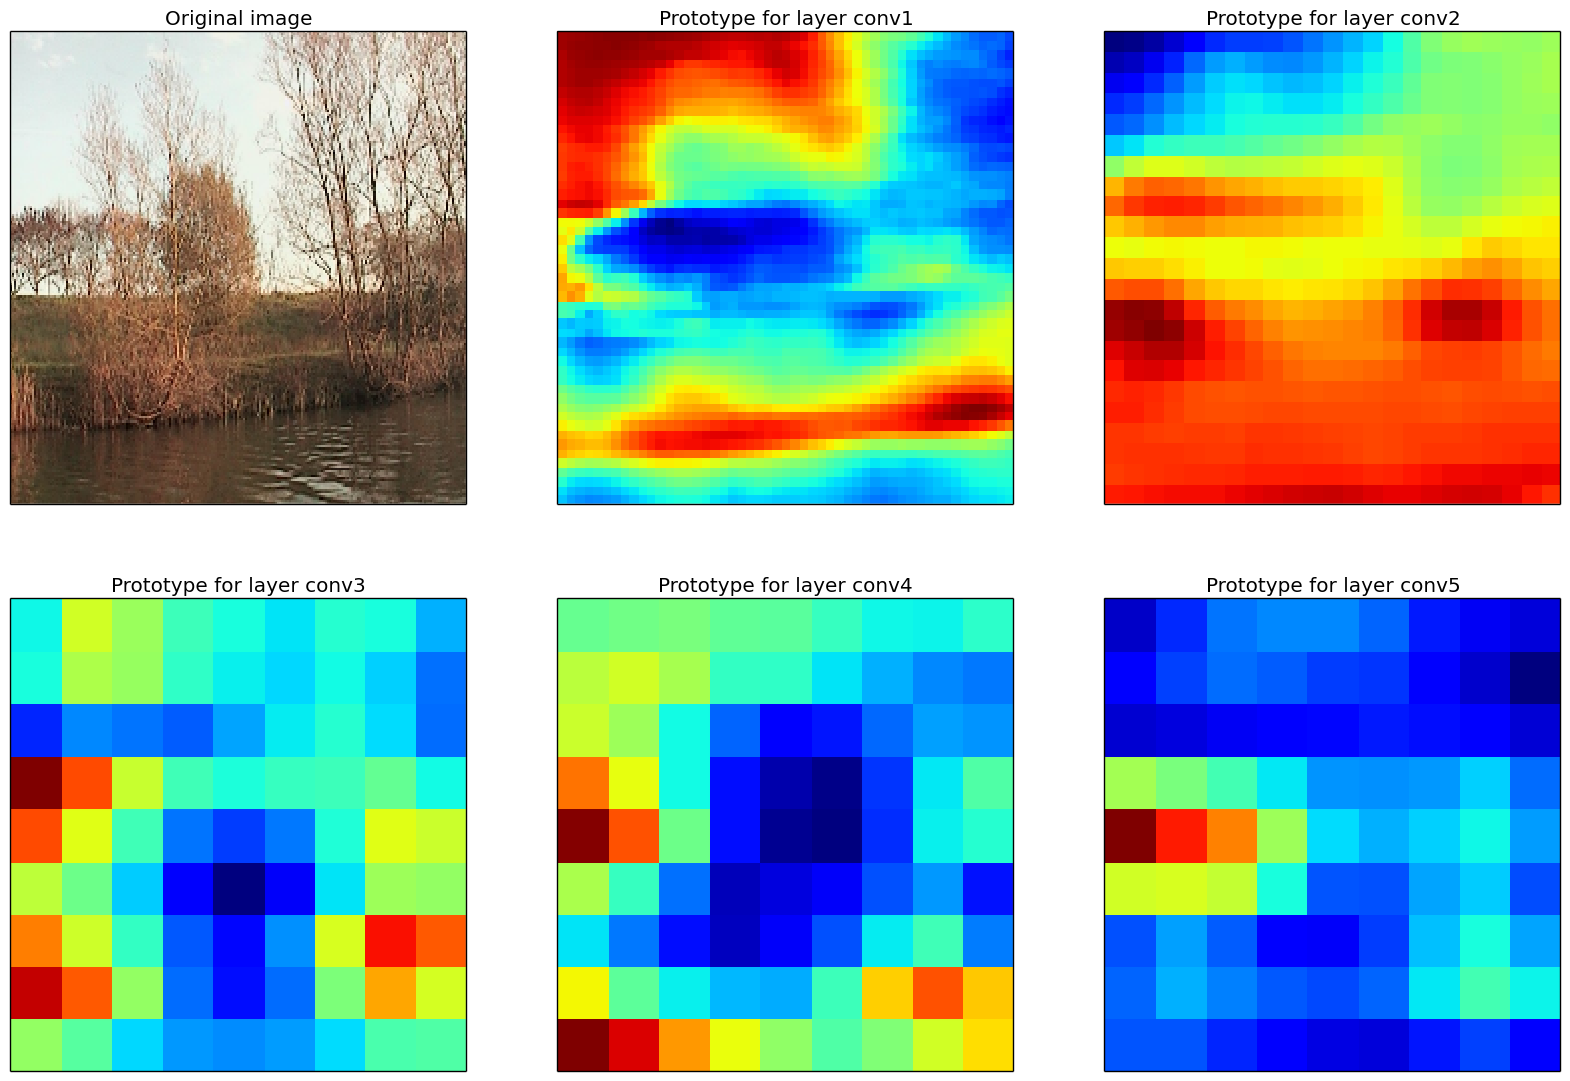
\includegraphics[width=0.8\linewidth]{images/classification/prototypes/avmaskplot7}}\\
\end{tabular}
\caption{Example of prototypes for a given image}
\label{prototypes}
\end{figure}

We generated prototypes for all classes, and tested whether an image can be recognized only using its class prototypes. Testing over a thousand random images and measuring using a cosine distance shows that all layers can be used as suitable descriptors, with distances to the wrong prototypes being indubitably larger than distances to the right prototype on average (see table~\ref{fulltrainvalues}, column 2 and 3 and fig.~\ref{allclft})

\begin{table}[htb]
\centering
\small
\begin{tabular}{|c|c|c||c|c|}
  \hline
  Layer & Overall Ratio & Precision (\%) & Ratio (seen)  & Ratio (unseen) \\
  & (complete dataset) & top-20 & ($1^{st}$ half dataset) & ($2^{nd}$ half dataset) \\
  \hline
  {\tt conv1} & 1.76 & 43.9\% & 1.70 & 1.03 \\ 
  {\tt conv2} & 2.99 & 42.3\% & 0.93 & 0.96 \\ 
  {\tt conv3} & 1.86 & 34.8\% & 1.40 & 0.94 \\ 
  {\tt conv4} & 1.79 & 08.4\% & 1.16 & 1.00 \\ 
  {\tt conv5} & 1.68 & 57.3\% & 1.32 & 0.98 \\ 
  {\tt pool5} & 1.86 & 52.0\% & 1.42 & 0.95 \\ 
  \hline
\end{tabular}
\caption{Ratio of median distance of a random image to the wrong prototypes over median distance to the correct prototype. $2^{nd}$ column refers to the ratio achieved using the complete dataset for training. $3^{rd}$ column give the percentage of successful top-20 classification using the distance to the prototypes of the full dataset. $4^{th}$ column is similar but using only half of the classes. $5^{th}$ column evaluate the generalization performance by evaluating images from the classes not used for training. }
\label{fulltrainvalues}
\end{table}

\begin{figure}[htb]
\centering
\begin{tabular}{ccc}
    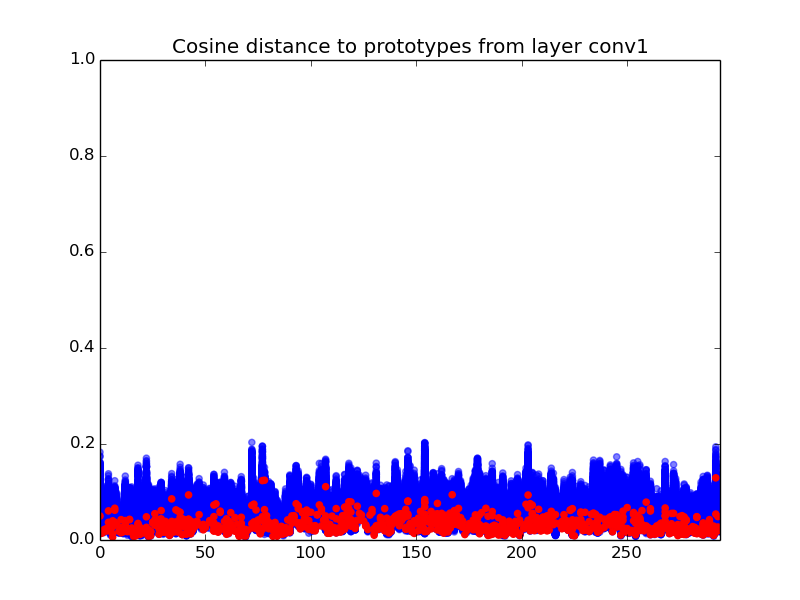
\includegraphics[width=0.3\linewidth]{images/classification/distances/all_classes_full_train/cos_distances_conv1}&
    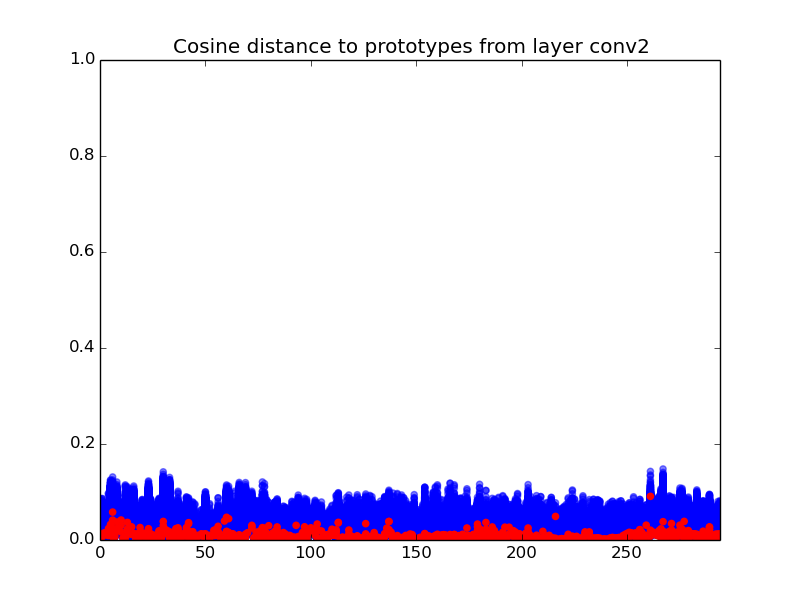
\includegraphics[width=0.3\linewidth]{images/classification/distances/all_classes_full_train/cos_distances_conv2}&
    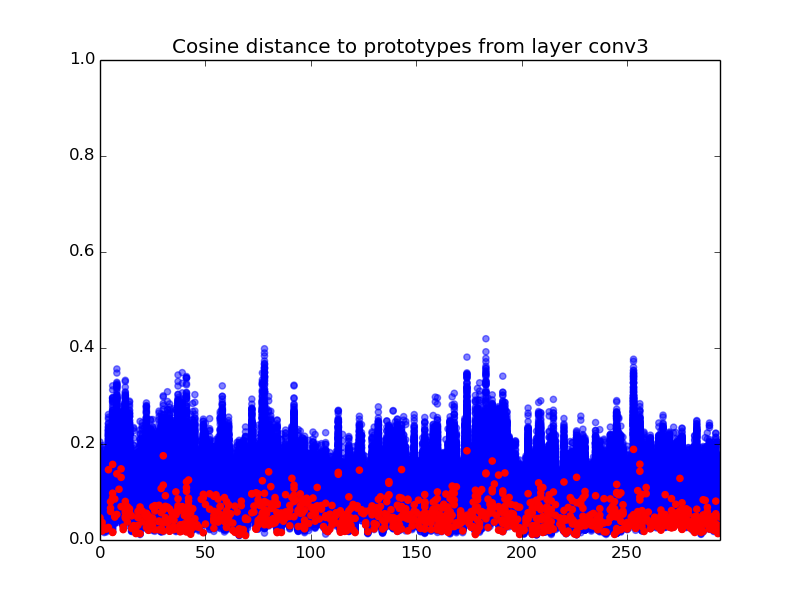
\includegraphics[width=0.3\linewidth]{images/classification/distances/all_classes_full_train/cos_distances_conv3} \\
    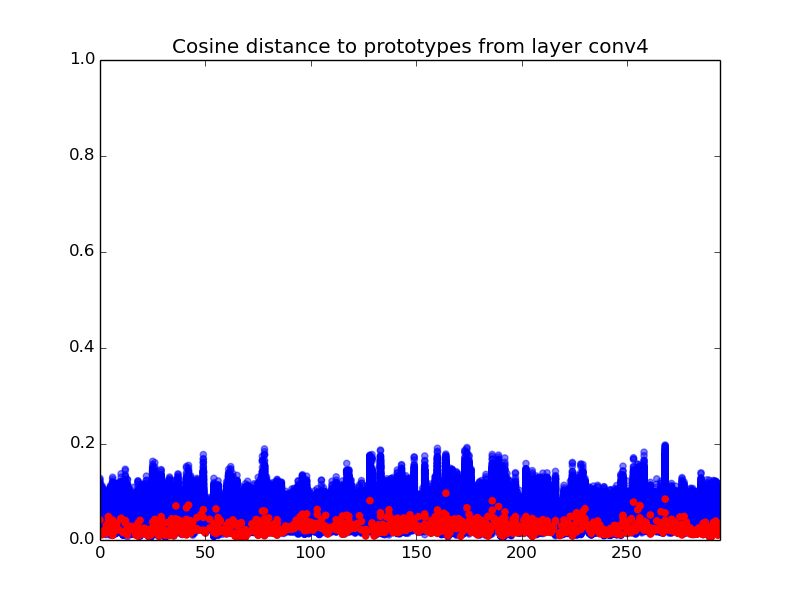
\includegraphics[width=0.3\linewidth]{images/classification/distances/all_classes_full_train/cos_distances_conv4}&
    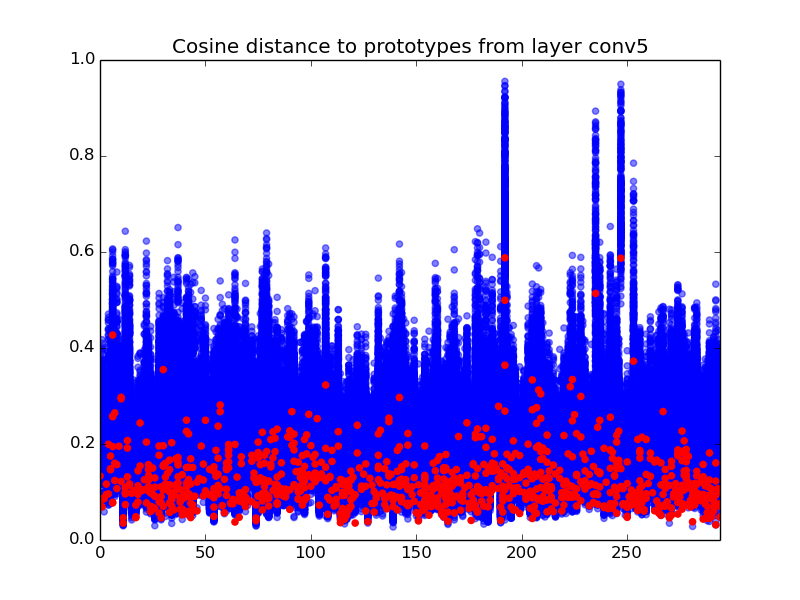
\includegraphics[width=0.3\linewidth]{images/classification/distances/all_classes_full_train/cos_distances_conv5}&
    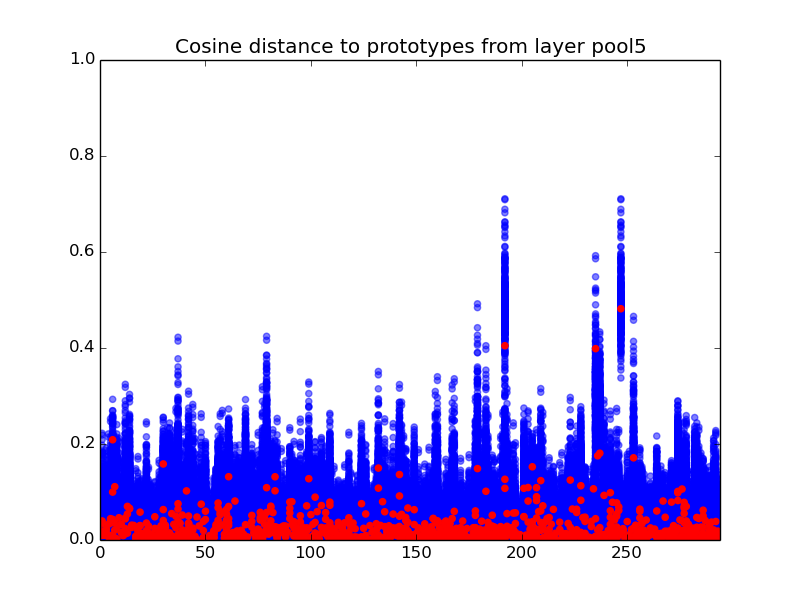
\includegraphics[width=0.3\linewidth]{images/classification/distances/all_classes_full_train/cos_distances_pool5} \\
\end{tabular}
\caption{Red dots represent the distance from a random class image to its class prototype, blue dots are distances to other class prototypes. Graphs show layers conv1 through pool5.}
\label{allclft}
\end{figure}

We also trained the same network on half the classes, to test for generalization capabilities. We wanted to test whether the network learned how to transform an image into its seasonal-invariant representation. %, proved to exist with the full training. % not idea what that means. CP
In the case of the classes observed in the training set, the representation results are analogous to the full dataset. However, the internal features are not discriminative when applied on images from unseen classes (table~\ref{fulltrainvalues}, column 4 and 5). It seems that the network learns how to efficiently discriminate between its known classes, rather than truly learning seasonal variations.

% Merged in table above
% \begin{table}[htb]
% \centering
% \begin{tabular}{|c|c|c|}
%   \hline
%    Layer & Ratio (seen) & Ratio (unseen) \\
%   \hline
%   conv1 & 1.70 & 1.03 \\
%   conv2 & 0.93 & 0.96 \\
%   conv3 & 1.40 & 0.94 \\
%   conv4 & 1.16 & 1.00 \\
%   conv5 & 1.32 & 0.98 \\
%   pool5 & 1.42 & 0.95 \\
%   \hline
% \end{tabular}
% \caption{Ratio of median distances, for seen and unseen classes}
% \label{halftrainvalues}
% \end{table}
